\section{Repetition/Introduction to Simulink/QuaRC}\label{sec:prob1}

\subsection{PID-(re)tuning}
The pre-tuned PID showed unsatisfactory performance and was re-tuned to better serve as the stable plant for the rest of the assignment. As pitch and elevation isn't very coupled, the two controllers were tuned independent of each other. The tuning was done in a manual fashion.

\begin{table}[hp]
	\centering
	\caption{Controller gains comparison}
	\begin{tabular}{llll}
		\hline
		Gain & Original & Improved \\
		\hline
		$K_{pp}$ & 93.2 & 14.0 \\
		$K_{pd}$ & 13.2 & 2.5 \\
		$K_{ei}$ & 2.3 & 2.3 \\
		$K_{ep}$ & 7.0 & 15.0 \\
		$K_{ed}$ & 10.0 & 13.0 \\
	\end{tabular}
	\label{tab:gains}
\end{table}

TODO: Step responses before and after tuning
%\begin{figure}[hp]
%	\centering
%		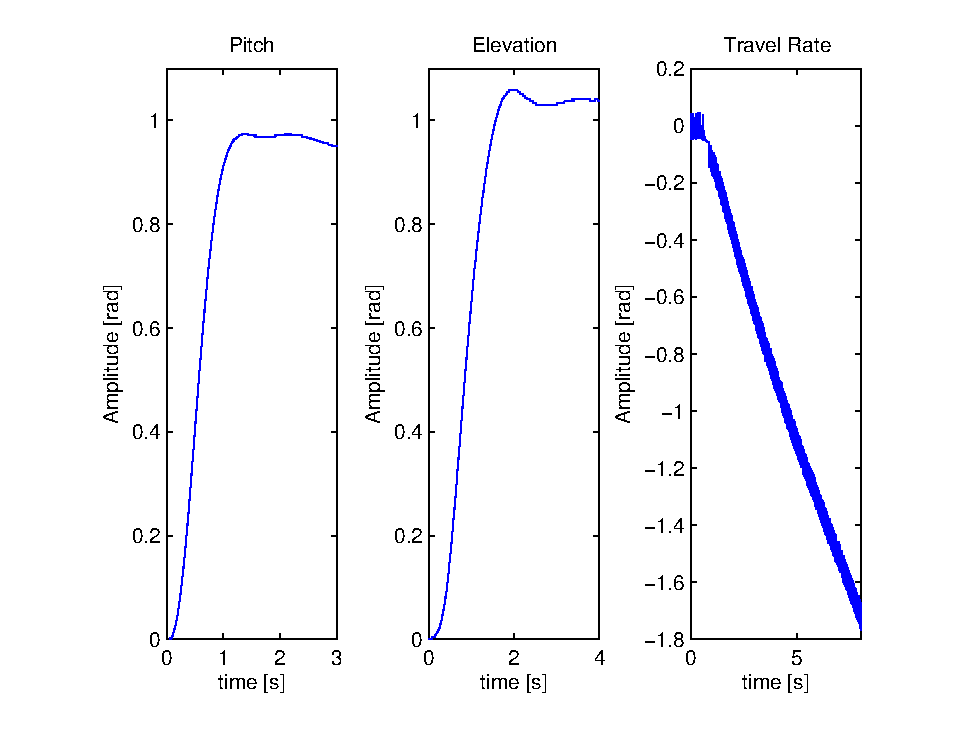
\includegraphics[width=0.9\textwidth]{figures/1/step_response.eps}
%	\caption{Step response.}
%	\label{fig:step_response}
%\end{figure}


\subsection{Model parameter estimation}
The measured parameters used in (\ref{eq:dynamics}) yielded a model with considerably different dynamics than the observed ones. The system identification toolbox in Matlab was therefore used to compute the parameters which fitted the recorded step responses. This was done by estimating the follow three step responses based on known input and recorded system behavior:

\begin{itemize}
	\item{Pitch setpoint to pitch}
	\item{Elevation setpoint to elevation}
	\item{Pitch to travel rate}
\end{itemize}

TODO: Step responses of both the actual system, and the newly identified awesome model.

\subsection{Results and discussion}

Figure \ref{fig:step_response} shows the pitch and elevation response to a step input, as well as the resulting travel rate to a step pitch input.
Would be nice to have a plot of the step responses with the original gains, to compare...



